%----------------------------------------------------------------------------
\chapter{\bevezetes}
%----------------------------------------------------------------------------


The digital era has led to large amounts of data being amassed by companies every day. Data comes from multiple sources: sensors, sales data, communication systems, logging of system events \etc. According to Forbes \cite{Forbes} 2.5 quintillion bytes of data created each day. That means 2.5 million Terabytes per day. Bigger corporations can easily create hundreds of Terabytes daily. We need a new solution to process this amount of data. The traditional relational databases (RDBMS) can deal only with Gigabytes. Hadoop provides a software framework to scale up our system for storing, processing and analyzing big data.

In this chapter, I will write about the basics of Hadoop architecture, why Hive was created on top if it and the performance issues it faces.

\section{Hadoop basics}
Apache Hadoop is an open source distributed framework for managing, processing  and storing a huge amount of data in clustered systems built from commodity hardware. All modules in Hadoop was designed with an assumption that hardware failures are common and should be automatically handled by the framework. One of the most important characteristic of Hadoop that it partitions the data and computation across many hosts and executing computation in parallel close to the data it uses.  \cite{Hadoop-wiki}

The base of the Hadoop framework contains the following modules:
\begin{itemize}
	\item HDFS - Hadoop Distributed File System: designed to store large data sets reliably and stream those at high bandwidth to user applications.
	\item Hadoop MapReduce: an implementation of the MapReduce programming model for large data processing
	\item YARN - Yet Another Resource Negotiator: a resource management and job scheduling technology
	\item Hadoop Common: contains libraries and utilities needed by other Hadoop modules
\end{itemize}
\subsection{Hadoop \vs traditional databases}
Traditional databases cannot be used when we want to process and store big data. Main differences between Hadoop and traditional RDBMS:
\begin{itemize}
	\item \textbf{Data Volume}: RDBMS works better when the data volume is low (Gigabytes). However when data size is huge (Terabytes-Petabytes) traditional databases fail. On the other hand Hadoop can easily handle this amount of data.
	\item \textbf{Data Variety}: this generally means the type of data to be processed. Hadoop has the ability to store and process data whether it is structured, semi-structured or unstructured. Even though  it is mostly used for large amount of unstructured data. 
	In contrast, traditional RDBMS can only be used to manage structured or semi-structured data. 
	\item \textbf{Scalability}: RDBMS provides vertical scalability. You can add more resources, memory or CPU to a machine in the cluster. Whereas Hadoop provides horizontal scalability. It means we can add more machines to an existing cluster. As a result of this Hadoop becomes fault tolerant. We can easily recover data in case of a failure of one of the machines.
	\item \textbf{Data Processing}: Apache Hadoop supports OLAP (Online Analytical Processing) that involves very complex queries and aggregations. The database design is de-normalized, having fewer tables. On the other hand, RDBMS supports OLTP (Online Transaction Processing), which involves fast query processing. The database design is normalized having large number of tables. \cite{Hadoop-vs-RDBMS}
\end{itemize}
\subsection{HDFS - Hadoop Distributed File System \cite{Shvachko:2010:HDF:1913798.1914427}}
HDFS is the file system of Hadoop. It stores file system metadata and application data separately. The dedicated server that stores metadata is the NameNode. Application data are stored on other servers (DataNodes). These servers are connected and they communicate using TCP-based protocols. 
\subsubsection*{NameNode \cite{Secondary-NameNode}}
NameNode keeps the directory tree of all files in the file system and tracks where file data is kept across the cluster. It does not store the files itself. Clients talk to the NameNode whenever they want to locate or add/move/copy/delete a file. The NameNode returns a list of relevant DataNode servers where the data is available. 

As a result of this approach, the NameNode is a Single Point of Failure in the HDFS cluster. Whenever the NameNode goes down, the file system becomes offline.
\begin{figure}[H]
	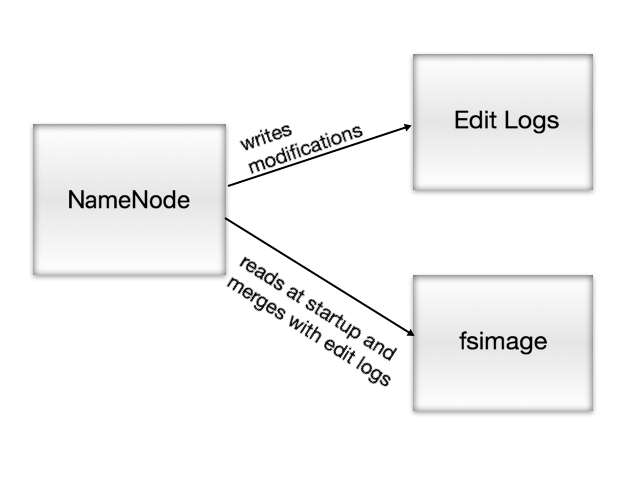
\includegraphics[width=80mm, keepaspectratio]{figures/namenode_problem.png}
	\centering
	\caption*{Problem with the NameNode}
\end{figure}
The image shows how NameNode stores information. There are two different files:
\begin{itemize}
	\item edit logs: the changes made to the file system after the NameNode started
	\item fsimage: a snapshot of the file system when the NameNode started
\end{itemize}
In production clusters the NameNode restarts are very rare. That means edit logs can grow large therefore in case of a crash we will lose huge amount of metadata since the fsimage is very old.

The Secondary NameNode helps to address this issue. It takes over the responsibility of merging the edit logs with fsimage. It collects edit logs on a regular basis and applies them to the fsimage. NameNode will use this fsimage in case of a crash and it can also be used to reduce the startup time of the NameNode.
It is important to remember that the Secondary NameNode is not a real backup NameNode it only merges the edits into the fsimage. 

\begin{figure}[H]
	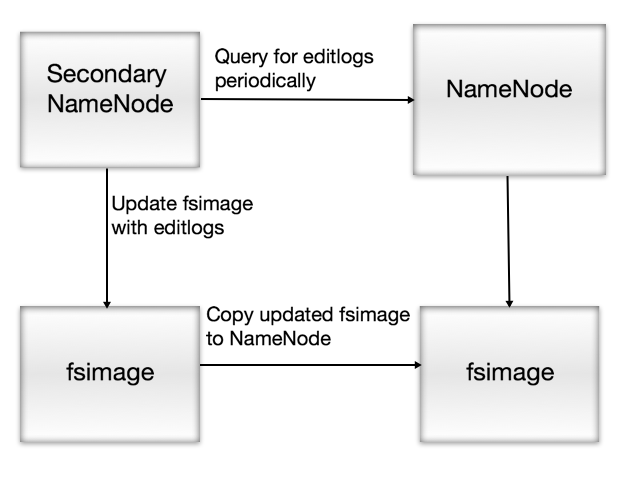
\includegraphics[width=80mm, keepaspectratio]{figures/secondary_namenode.png}
	\centering
	\caption*{Solution using the Secondary NameNode}
\end{figure}

\subsubsection*{DataNodes}
On a DataNode a block is represented by two files on the host's native file system. The first contains the data itself, the second is the metadata: checksum for the data and generation stamp. 

On startup, the DataNodes connect to the NameNode and perform a handshake. The reason for the handshake, is to verify the namespace ID and software version of the DataNodes. If one of them does not match with the NameNode's value, the DataNode automatically shuts down. After a successful handshake the DataNode registers with the NameNode. DataNode will store it's internal identifier persistently. This way, if restart occurs the DataNodes will be recognizable even if they get a different IP address or port. After the ID is registered to the NameNode the ID of a DataNode will never change. 

 When a DataNode is registered it sends a block report immediately. It contains  block id, generation stamp and the length of each block the DataNode server hosts. To provide up-to-date information to the NameNode reports are sent every hour. 

During normal operation, DataNodes send heartbeats to the NameNode. It ensures the NameNode that the DataNode is operating and block replicas of the server are available. If the NameNode does not receive a heartbeat from a DataNode it will consider the node to be out of service. The default heartbeat interval is three seconds.

\subsubsection*{HDFS Client}
User applications access the file system using the HDFS client. It exports the HDFS file system interface. Similar to a traditional file system, HDFS supports operations to read, write and delete files and to create or delete directories. The user references files and directories by paths in the namespace. 

When someone reads a file, HDFS Client asks the NameNode for the list of DataNodes that host replicas of the blocks of the file. Then it will directly contacts the DataNode and request the desired block. When the client writes, it asks the NameNode to choose DataNodes to host replicas of the first block of the file. When the first block is filled, the client requests for new DataNodes to place the next blocks.

\begin{figure}[H]
	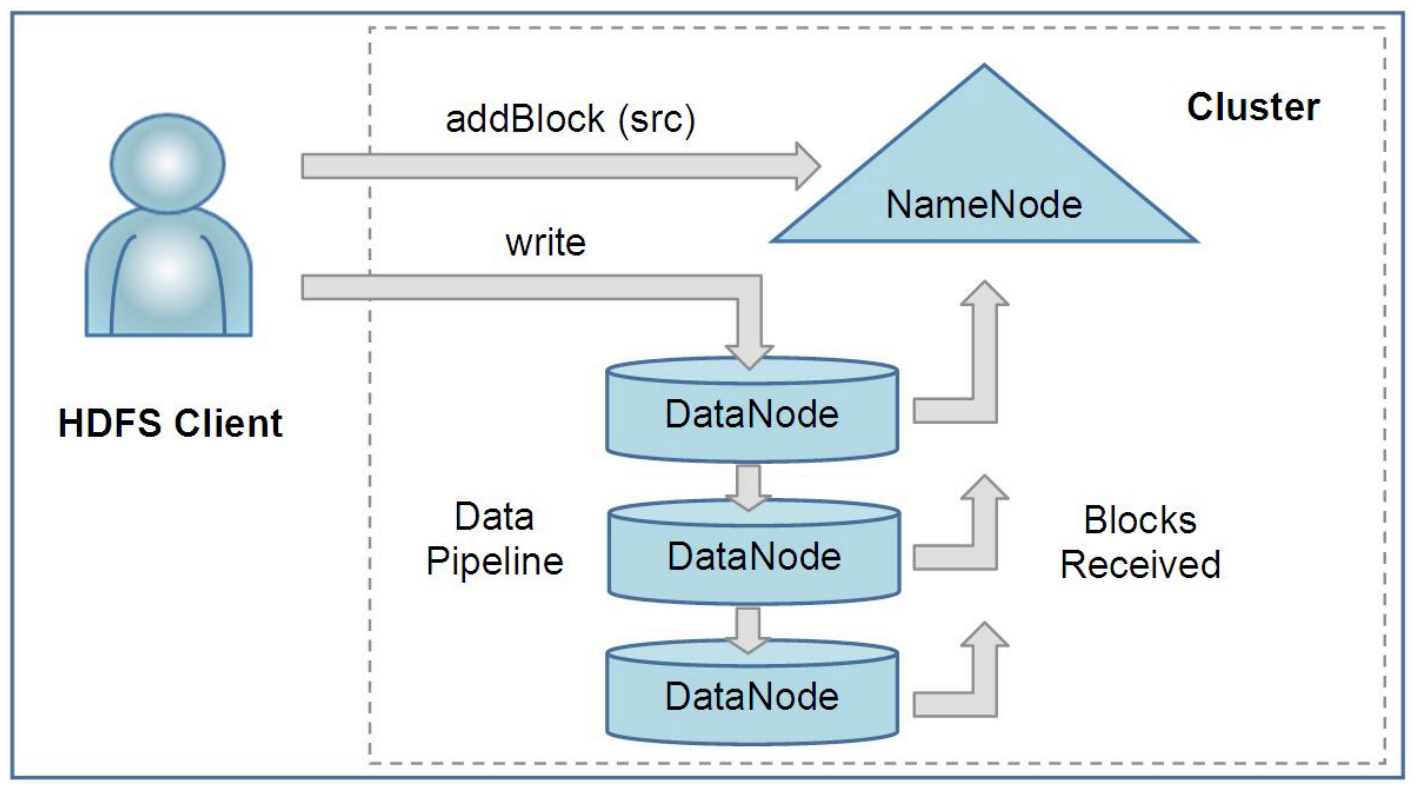
\includegraphics[width=100mm, keepaspectratio]{figures/hdfs_client.png}
	\centering
\end{figure}
The client creates a new file by giving its path to the NameNode. For each block, the NameNode will return a list of DataNodes to place the replicas. The client pipelines data to the given DataNodes, and they will confirm the creation of the block to the NameNode.
\subsection{MapReduce \cite{Dean:2004:MSD:1251254.1251264}}
MapReduce is a programming model for processing and generating large data sets. Users specify two functions:
\begin{itemize}
	\item map function: processes a key/value pair to generate a set of intermediate key/value pairs
	\item reduce function: merges the intermediate values associated with the same key
\end{itemize}

Programs written in this style are automatically executed parallelly  on large clusters. This allows programmers with no experience in parallel programming and distributed systems to take advantage of the available resources on the cluster.
\paragraph{Example \cite{MapReduce-example}}
This example shows how MapReduce handles the problem of counting words. We have the following list of words: 
\begin{center}
	\textbf{Dear, Bear, River, Car, Car, River, Deer, Car, Bear}
\end{center}

\begin{figure}[H]
	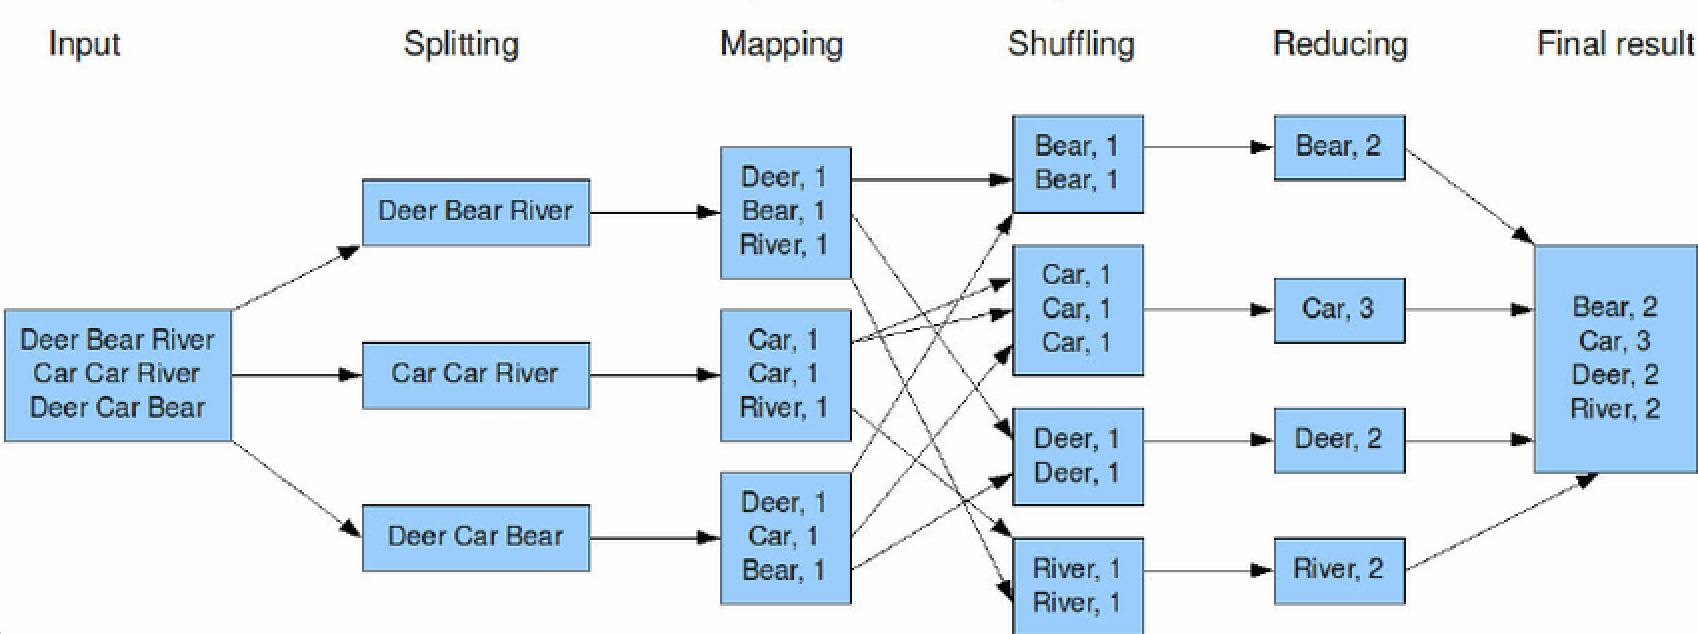
\includegraphics[width=150mm, keepaspectratio]{figures/MapReduce_Example.png}
	\caption*{The overall MapReduce word count process}
	\centering
\end{figure}
\begin{itemize}
	\item \textbf{Splitting}: the first step is dividing the input into three splits. This will distribute the work among the Map nodes.
	\item \textbf{Mapping}: tokenize the words in each mapper and giving a value of 1 for each token/word, since every word in itself will occur once.
	\item \textbf{Shuffling}: after the mapping phase a partition process takes place where sorting and shuffling happens: all key-value pairs with the same key will be sent to the corresponding reducer
	\item \textbf{Reducing}: a reducer gets the list of pairs and counts the number of ones in this list.
\end{itemize}

\subsubsection*{Advantages of MapReduce}
\paragraph{Parallel processing}
In MapReduce we are dividing the job among multiple nodes, that can work on a part of the job simultaneously. This way the data processing is done by multiple machines instead of one, so the processing time is reduced.
\paragraph{Data locality}
In Hadoop MapReduce, instead of moving data into the processing unit, we move the processing unit to the data. The traditional approach has its limit when it comes to processing big data. Moving huge data to  processing is costly, network issues can occur and the master node (where data is stored) can get overloaded and may fail. 

However, the MapReduce approach is very cost efficient, since all the nodes are working parallel on their part of the data and there is no chance of a node getting overloaded.

Using Hadoop we just need to provide the map and reduce funtions in java, the rest is done by the framework.  The word count example would look like the following in java:
\paragraph{Map}\mbox{}\\
\begin{lstlisting}[language=Java]
	public void map(LongWritable key, Text value, Context context) throws OException,InterruptedException {
		String line = value.toString();
		StringTokenizer tokenizer = new StringTokenizer(line);
		while (tokenizer.hasMoreTokens()) {
			value.set(tokenizer.nextToken());
			context.write(value, new IntWritable(1));
		}
	}
\end{lstlisting}
Both the input and output of the Mapper is a key/value pair. 

Input:
\begin{itemize}
	\item Key: the offset of each line in the text file: LongWritable
	\item Value: each individual line: Text
\end{itemize}

Output:
\begin{itemize}
	\item Key: the tokenized words: Text
	\item Value: the hardcoded value 1: IntWritable
\end{itemize}

\paragraph{Reduce}\mbox{}\\
\begin{lstlisting}
	public void reduce(Text key, Iterable<IntWritable> values,Context context) throws IOException,InterruptedException {
		int sum=0;
		for(IntWritable x: values) {
			sum+=x.get();
		}
		context.write(key, new IntWritable(sum));
	}
\end{lstlisting}
Both the input and output of the Mapper is a key/value pair. 

Input:
\begin{itemize}
	\item Key: unique words which have been generated after the sorting and shuffling phase: Text
	\item Value: a list of integers corresponding to each key: IntWritable 
	\item \eg Bear, [1, 1]
\end{itemize}

Output:
\begin{itemize}
	\item Key: all the unique words present in the input text file: Text
	\item Value: the number of occurrences of each of the unique words: IntWritable 
	\item \eg  Bear, 2; Car, 3
\end{itemize}

The traditional way to execute MapReduce operations is that the users specify the Map and Reduce functions in Java. However, this approach has some problems:
\begin{itemize}
	\item it is not a high level language for data processing
	\item data scientists do not understand Java. They came from the world of traditional databases, where SQL is used.
	\item even a simple problem (like word counting) resulted in hundreds of lines of code.
\end{itemize}

\subsection{Yarn \cite{YARN}}
\subsubsection*{Hadoop 1.0 resource management}
Previous to Hadoop 2.0, a single JobTracker had the responsibility to monitor the resources and distribute the MapReduce jobs for the DataNodes and monitor these jobs. 

In Hadoop 1.0 the MapReduce module was responsible for cluster resource management and data processing as well.

\begin{figure}[H]
	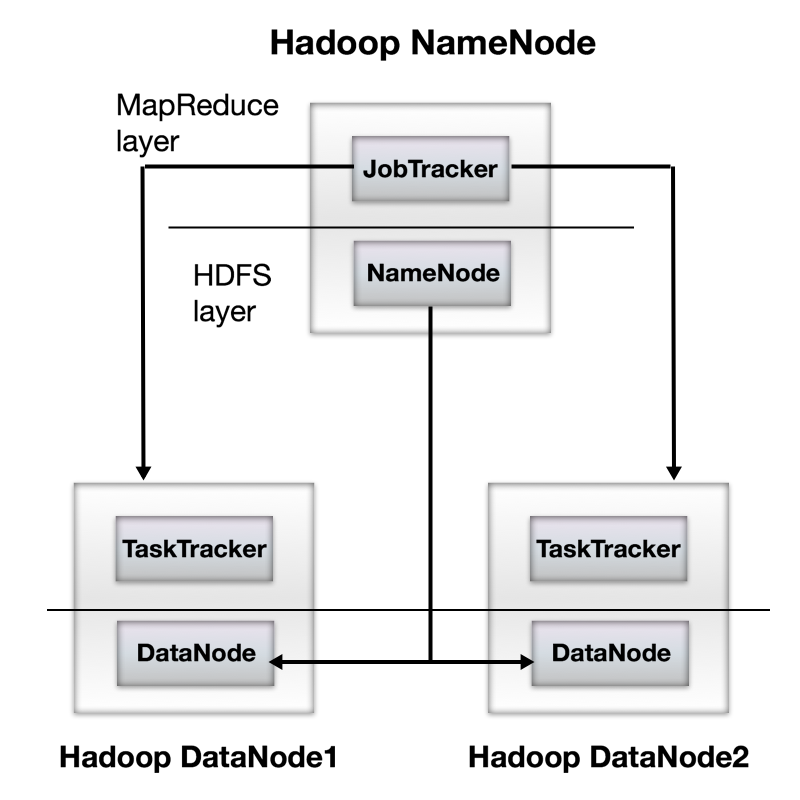
\includegraphics[width=100mm, keepaspectratio]{figures/hadoop10.png}
	\centering
	\caption*{Hadoop 1.0 architecture}
	\centering
\end{figure}

Resource management in Hadoop 1.0 \cite{Hadoop1.0}:
\begin{enumerate}
\item Client applications submit jobs to the Job tracker.
\item The JobTracker talks to the NameNode to determine the location of the data
\item The JobTracker locates TaskTracker nodes with available slots at or near the data
\item The JobTracker submits the work to the chosen TaskTracker nodes.
\item The TaskTracker nodes are monitored. If they do not submit heartbeat signals often enough, they are deemed to have failed and the work is scheduled on a different TaskTracker.
\item A TaskTracker will notify the JobTracker when a task fails. The JobTracker decides what to do then: it may resubmit the job elsewhere, it may mark that specific record as something to avoid, and it may even blacklist the TaskTracker as unreliable.
\item When the work is completed, the JobTracker updates its status.
\item Client applications can poll the JobTracker for information.
\end{enumerate}

The architecture of Hadoop 1.0 has many problems:
\begin{itemize}
	\item  It \textbf{limits scalability} since the JobTracker runs on a single machine doing multiple tasks it becomes a bottleneck: resource management, job and task scheduling, monitoring are done by the JobTracker.
	\item JobTracker is a \textbf{Single Point of Failure}. If it goes down, all the jobs are halted.
	\item In Hadoop 1.0 \textbf{JobTracker is tightly integrated with the MapReduce} module so only MapReduce applications can run on Hadoop. Altough MapReduce is powerful enough to express many data analysis algorithms (mostly batch driven data analysis), it is not always the optimal paradigm. It is often desirable to run other computation paradigms on Hadoop like real time analysis and Message-Passing approach, \etc. Since HDFS makes it easy to store large amounts of data it is desirable to utilize this for other big data problems.
\end{itemize}

Developers recognized that splitting the responsibility to resource management and application monitoring has serious benefits. YARN is a re-architecture of Hadoop that allows multiple applications to run on the same platform. With YARN, applications run "in" Hadoop, instead of "on" Hadoop. This takes Hadoop beyond a batch application to a ‘data operating system’ where HDFS is the file system and YARN is the operating system. 

\begin{figure}[H]
	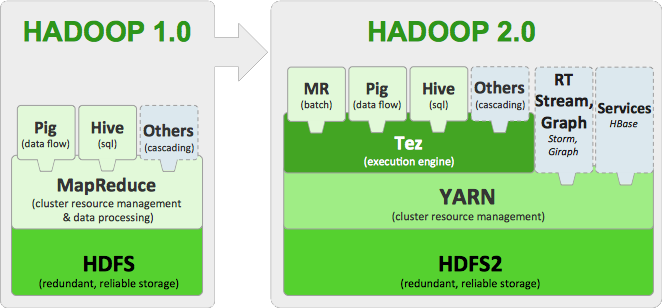
\includegraphics[width=100mm, keepaspectratio]{figures/hadoop10vs20.png}
	\centering
	\caption*{From Hadoop 1.0 to Hadoop 2.0}
	\centering
\end{figure}

The fundamental idea of YARN is to split up the functionalities of resource management and job scheduling/monitoring. In YARN we have a global ResourceManager (RM) and per-application ApplicationMaster (AM). An application is either a single job or a DAG (Directed Acyclic Graph) of jobs. 

The \textbf{ResourceManager} and the \textbf{NodeManager} together form the data-processing framework. ResourceManager distributes the resources among all the applications in the system. The NodeManager is a per-machine agent who is responsible for containers, monitor their resource usages (cpu, memory, network, disk) and report them to the ResourceManager. 

The per-application \textbf{ApplicationMaster} is framework specific, and its task is to ask the ResourceManager for resources when needed. It is also working with the NodeManager to execute and monitor tasks.

The ResourceManager has two main components: Scheduler and ApplicationsManager.
\begin{itemize}
	\item The Scheduler is responsible for allocating resources to various applications running in the cluster. The scheduler schedules based on the resource requirements of each application. The scheduler does not perform monitoring or status tracking of the application. 
	\item The ApplicationsManager is responsible for accepting job-submissions. It negotiates the first container for executing the application specific ApplicationMaster. It also provides a service for restarting the ApplicationMaster container on failure. 
\end{itemize}

\begin{figure}[H]
	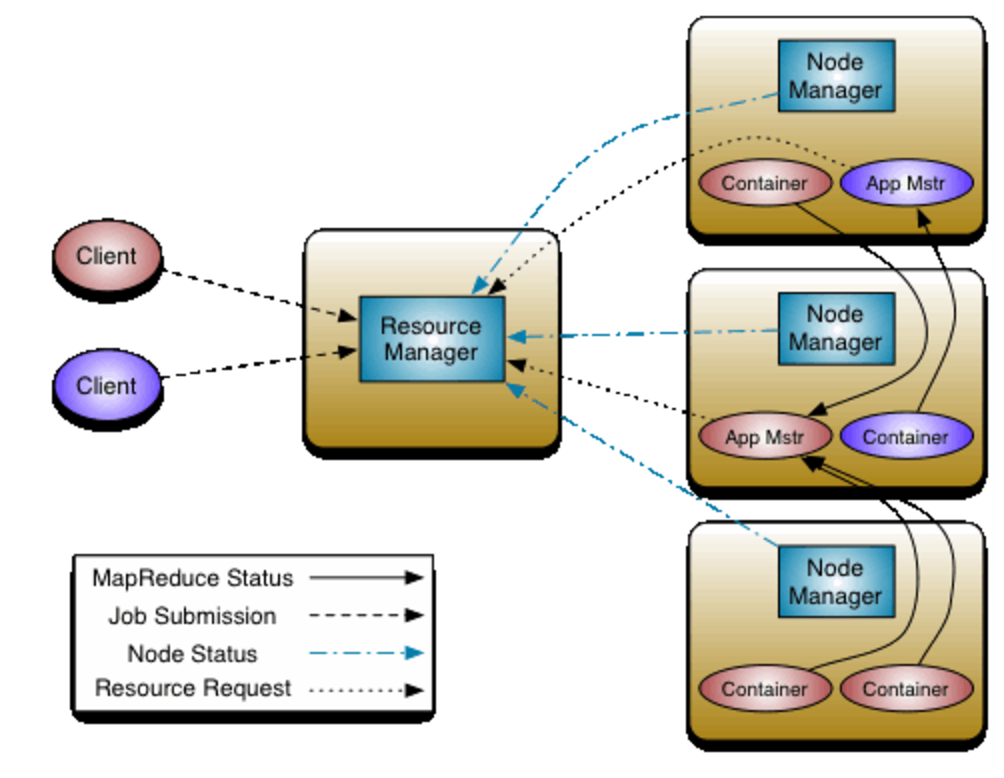
\includegraphics[width=120mm, keepaspectratio]{figures/yarn.png}
	\centering
	\caption*{Yarn architecture}
	\centering
\end{figure}

In summary, with YARN Hadoop is able to run applications that do not follow the MapReduce modell since it decouples the resource management and scheduling capabilities of MapReduce. With the help of YARN we can efficiently utilize the resources and can run multiple applications in Hadoop, all sharing a common resource.